\documentclass[12pt,letterpaper]{exam}
\usepackage[lmargin=1in,rmargin=1in,tmargin=1in,bmargin=1in]{geometry}
\usepackage{../style/exams}

% -------------------
% Course & Exam Information
% -------------------
\newcommand{\course}{MAT 100: Exam 2}
\newcommand{\term}{Fall -- 2021}
\newcommand{\examdate}{12/13/2021}
\newcommand{\timelimit}{85 Minutes}

\setbool{hideans}{false} % Student: True; Instructor: False

% -------------------
% Content
% -------------------
\begin{document}

\examtitle
\instructions{Write your name on the appropriate line on the exam cover sheet. This exam contains \numpages\ pages (including this cover page) and \numquestions\ questions. Check that you have every page of the exam. Answer the questions in the spaces provided on the question sheets. Be sure to answer every part of each question and show all your work.} 
\scores
\bottomline
\newpage

% ---------
% Questions
% ---------
\begin{questions}

% Question 1
\newpage
\question[5] Sketch the quadratic function $f(x)= 4 - (x + 3)^2$ in the graph below. Your sketch should include the vertex and axis of symmetry for $f(x)$. 
	\[
	\fbox{
	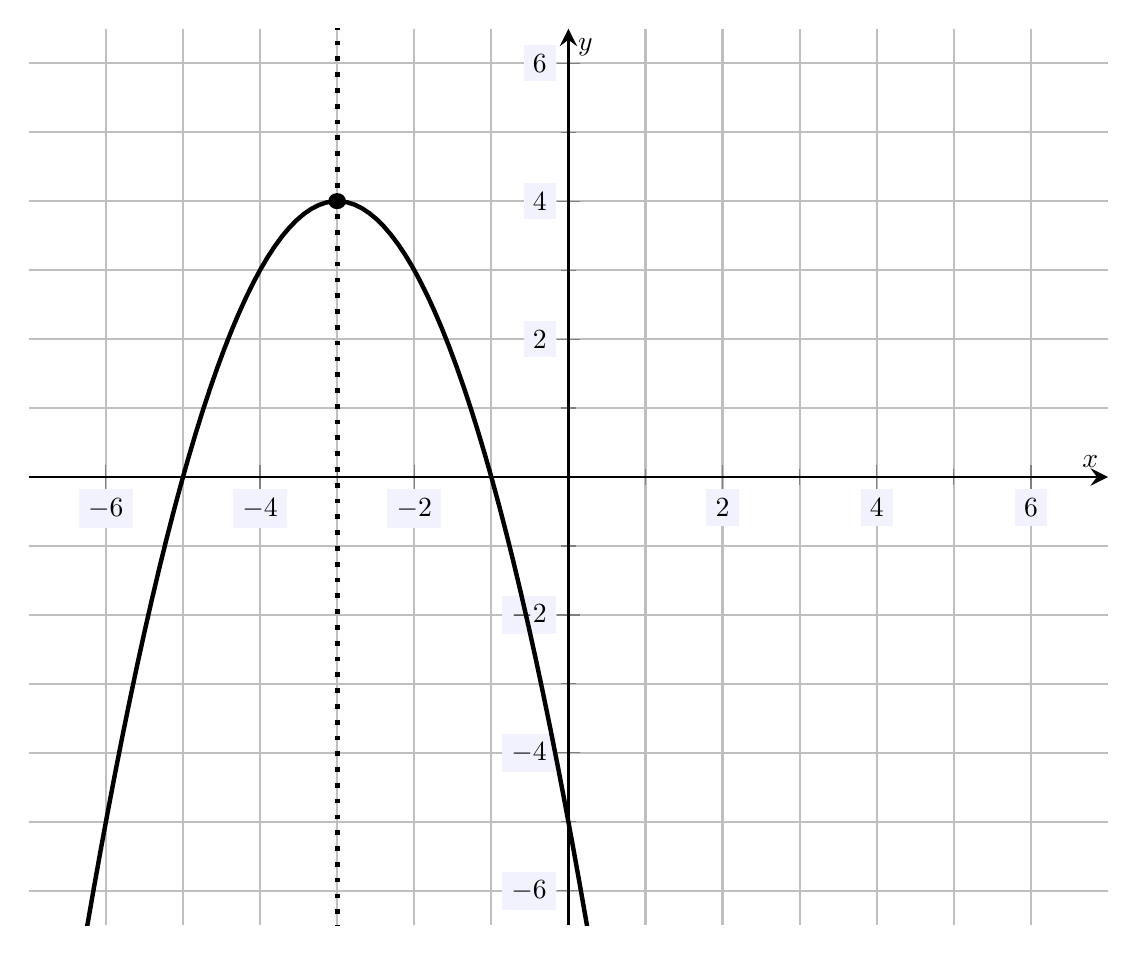
\begin{tikzpicture}[scale=2,every node/.style={scale=0.5}]
	\begin{axis}[
	grid=both,
	axis lines=middle,
	ticklabel style={fill=blue!5!white},
	xmin= -7, xmax=7,
	ymin= -6.5, ymax=6.5,
	xtick={-6,-4,-2,0,2,4,6},
	ytick={-6,-4,-2,0,2,4,6},
	minor tick = {-5,-3,...,5},
	xlabel=\(x\),ylabel=\(y\),
	]
	\addplot[thick, domain= -7:7,samples=150] {4 - (x + 3)^2};
	\draw[dotted,line width= 0.03cm] (-3,-10) -- (-3,10);
	\draw[fill=black] (-3,4) circle (0.1);
	\end{axis}
	\end{tikzpicture}
	}
	\] \pspace

{\noindent\itshape From the form of the function $f(x)= 4 - (x + 3)^2$, we can immediately see that the vertex is $(-3, 4)$ and that the parabola opens downwards.}





% Question 2
\newpage
\question[10] Let $f(x)$ be the quadratic function $f(x)= 5x^2 + 10x - 7$.
\begin{enumerate}[(a)]
\item Find the vertex and axis of symmetry for $f(x)$.
\item Does this parabola open upwards or downwards? Explain.
\item Is the function convex or concave? 
\item Does the function have a maximum or minimum value? Explain. 
\item Find the maximum or minimum value from (d). 
\end{enumerate} \pspace

{\noindent\bfseries Solution.}
\begin{enumerate}[(a)]
{\itshape
\item We know that the $x$-coordinate of the vertex is\dots
	\[
	x= \dfrac{-b}{2a}= \dfrac{-10}{2(5)}= \dfrac{-10}{10}= -1
	\]
The $y$-coordinate of the vertex is $f(-1)= 5(-1)^2 + 10(-1) - 7= 5 - 10 - 7= -12$. Therefore, the vertex is $(-1, -12)$. It is also immediate that the axis of symmetry is $x= -1$. 
	
	\[
	\boxed{%
	\begin{aligned}
	\text{Vertex: }& (-1, -12) \\
	\text{Axis of Symmetry: }& x= -1
	\end{aligned}
	}
	\] \pspace

\item Because $a= 5 > 0$, the parabola opens upwards. \pspace

\item Because the parabola opens upwards, the function is convex. \pspace

\item Because the parabola opens upwards, the function has a minimum. \pspace

\item We know the minimum value occurs at the vertex. The vertex has coordinate $(-1, -12)$. Therefore, the minimum value is $-12$. 
}
\end{enumerate}





% Question 3
\newpage
\question[5] Find the vertex form of $y= x^2 - 8x + 21$. \pspace

{\noindent\itshape We complete the square. Observe that $\frac{1}{2} \cdot -8= -4$ and that $(-4)^2= 16$. Then\dots}
	\[
	\begin{aligned}
	y&= x^2 - 8x + 21 \\[0.3cm]
	y&= x^2 - 8x + (16 - 16) + 21 \\[0.3cm]
	y&= (x^2 - 8x + 16) + (-16 + 21) \\[0.3cm]
	y&= (x - 4)^2 + 5
	\end{aligned}
	\] \pspace
	
	\[
	\boxed{y= (x - 4)^2 + 5}
	\]





% Question 4
\newpage
\question[5] Factor the polynomial $x^2 - 16x + 55$. \pspace

	\begin{table}[!ht]
	\centering
	\underline{\bfseries 55} \pvspace{0.2cm}
	\begin{tabular}{rr}
	$1 \cdot 55$ & $56$ \\
	$-1 \cdot -55$ & $-56$ \\
	$5 \cdot 11$ & $16$ \\ \hline
	\multicolumn{1}{|r}{$-5 \cdot -11$} & \multicolumn{1}{r|}{$-16$} \\ \hline
	\end{tabular}
	\end{table}

	\[
	x^2 - 16x + 55= (x - 5)(x - 11)
	\] \pspace
	
	\[
	\boxed{(x - 11)(x - 5)}
	\]





% Question 5
\newpage
\question[5] Factor the polynomial $x^2 - 2x - 48$. \pspace

	\begin{table}[!ht]
	\centering
	\underline{\bfseries 48} \pvspace{0.2cm}
	\begin{tabular}{rr}
	$1 \cdot -48$ & $-47$ \\
	$-1 \cdot 48$ & $47$ \\
	$2 \cdot -24$ & $-22$ \\
	$-2 \cdot 24$ & $22$ \\
	$3 \cdot -16$ & $-13$ \\
	$-3 \cdot 16$ & $13$ \\
	$4 \cdot -12$ & $-8$ \\
	$-4 \cdot 12$ & $8$ \\ \hline
	\multicolumn{1}{|r}{$6 \cdot -8$} & \multicolumn{1}{r|}{$-2$} \\ \hline
	$-6 \cdot 8$ & $2$ \\
	\end{tabular}
	\end{table}

	\[
	x^2 - 2x - 48= (x + 6)(x - 8)
	\] \pspace
	
	\[
	\boxed{(x - 8)(x + 6)}
	\]





% Question 6
\newpage
\question[5] Factor the polynomial $2x^2 + 7x - 30$. \pspace

	\[
	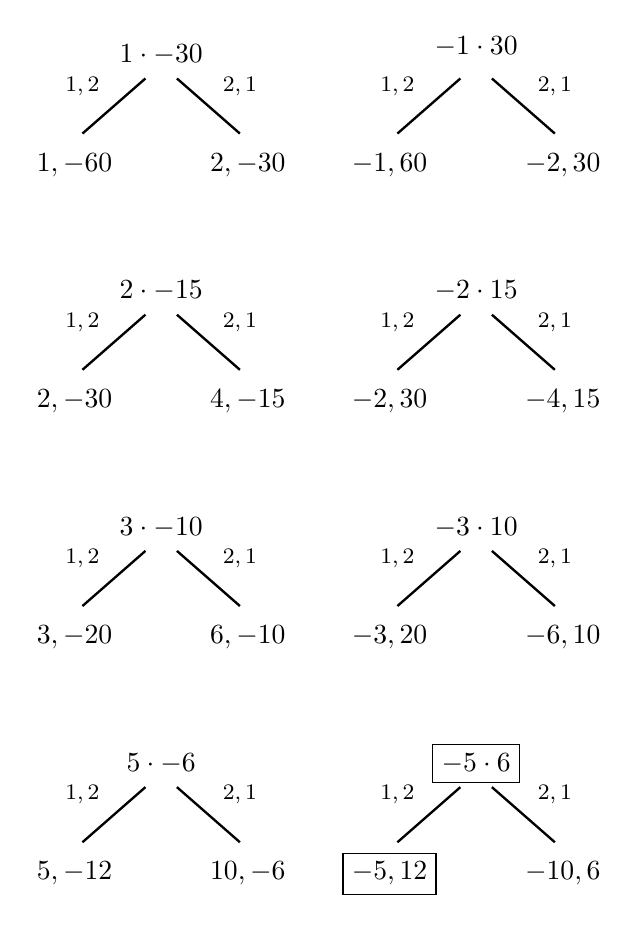
\begin{tikzpicture}
	\node at (0,0) {$1 \cdot -30$};
	\node at (-1.0,-0.4) {\footnotesize$1, 2$};
	\draw[line width=0.03cm,label={1}] (-0.2,-0.3) -- (-1,-1);
	\node at (-1.1,-1.4) {$1, -60$};
	\node at (1.0,-0.4) {\footnotesize$2, 1$};
	\draw[line width=0.03cm] (0.2,-0.3) -- (1,-1);
	\node at (1.1,-1.4) {$2, -30$};	
	
	\tikzset{shift={(4,0)}}

	\node at (0,0.1) {$-1 \cdot 30$};
	\node at (-1.0,-0.4) {\footnotesize$1, 2$};
	\draw[line width=0.03cm,label={1}] (-0.2,-0.3) -- (-1,-1);
	\node at (-1.1,-1.4) {$-1, 60$};
	\node at (1.0,-0.4) {\footnotesize$2, 1$};
	\draw[line width=0.03cm] (0.2,-0.3) -- (1,-1);
	\node at (1.1,-1.4) {$-2, 30$};
	
	\tikzset{shift={(-4,-3)}}
	
	\node at (0,0) {$2 \cdot -15$};
	\node at (-1.0,-0.4) {\footnotesize$1, 2$};
	\draw[line width=0.03cm,label={1}] (-0.2,-0.3) -- (-1,-1);
	\node at (-1.1,-1.4) {$2, -30$};
	\node at (1.0,-0.4) {\footnotesize$2, 1$};
	\draw[line width=0.03cm] (0.2,-0.3) -- (1,-1);
	\node at (1.1,-1.4) {$4, -15$};
	
	\tikzset{shift={(4,0)}}

	\node at (0,0) {$-2 \cdot 15$};
	\node at (-1.0,-0.4) {\footnotesize$1, 2$};
	\draw[line width=0.03cm,label={1}] (-0.2,-0.3) -- (-1,-1);
	\node at (-1.1,-1.4) {$-2, 30$};
	\node at (1.0,-0.4) {\footnotesize$2, 1$};
	\draw[line width=0.03cm] (0.2,-0.3) -- (1,-1);
	\node at (1.1,-1.4) {$-4, 15$};

	\tikzset{shift={(-4,-3)}}
	
	\node at (0,0) {$3 \cdot -10$};
	\node at (-1.0,-0.4) {\footnotesize$1, 2$};
	\draw[line width=0.03cm,label={1}] (-0.2,-0.3) -- (-1,-1);
	\node at (-1.1,-1.4) {$3, -20$};
	\node at (1.0,-0.4) {\footnotesize$2, 1$};
	\draw[line width=0.03cm] (0.2,-0.3) -- (1,-1);
	\node at (1.1,-1.4) {$6, -10$};
	
	\tikzset{shift={(4,0)}}

	\node at (0,0) {$-3 \cdot 10$};
	\node at (-1.0,-0.4) {\footnotesize$1, 2$};
	\draw[line width=0.03cm,label={1}] (-0.2,-0.3) -- (-1,-1);
	\node at (-1.1,-1.4) {$-3, 20$};
	\node at (1.0,-0.4) {\footnotesize$2, 1$};
	\draw[line width=0.03cm] (0.2,-0.3) -- (1,-1);
	\node at (1.1,-1.4) {$-6, 10$};

	\tikzset{shift={(-4,-3)}}
	
	\node at (0,0) {$5 \cdot -6$};
	\node at (-1.0,-0.4) {\footnotesize$1, 2$};
	\draw[line width=0.03cm,label={1}] (-0.2,-0.3) -- (-1,-1);
	\node at (-1.1,-1.4) {$5, -12$};
	\node at (1.0,-0.4) {\footnotesize$2, 1$};
	\draw[line width=0.03cm] (0.2,-0.3) -- (1,-1);
	\node at (1.1,-1.4) {$10, -6$};
	
	\tikzset{shift={(4,0)}}

	\node at (0,0) {\framebox{$-5 \cdot 6$}};
	\node at (-1.0,-0.4) {\footnotesize$1, 2$};
	\draw[line width=0.03cm,label={1}] (-0.2,-0.3) -- (-1,-1);
	\node at (-1.1,-1.4) {\framebox{$-5, 12$}};
	\node at (1.0,-0.4) {\footnotesize$2, 1$};
	\draw[line width=0.03cm] (0.2,-0.3) -- (1,-1);
	\node at (1.1,-1.4) {$-10, 6$};
	\end{tikzpicture}
	\]

	\[
	2x^2 + 7x - 30= (2x - 5)(x + 6)
	\] \pspace
	
	\[
	\boxed{(2x - 5)(x + 6)}
	\]





% Question 7
\newpage
\question[5] Consider the function $f(x)= x^2 + 2x - 8$. Find the $x$ and $y$ intercepts for this function. \pspace

{\noindent\itshape The $y$-intercept occurs when $x= 0$. But then $y= f(0)= 0^2 + 2(0) - 8= 0 + 0 - 8= -8$. Therefore, the $y$-intercept is $(0, -8)$. \pspace

The $x$-intercepts occur when $y= 0$. But then $x^2 + 2x - 8= 0$. Observe\dots
	\[
	\begin{aligned}
	x^2 + 2x - 8&= 0 \\
	(x - 2)(x + 4)&= 0
	\end{aligned}
	\]
But then either $x - 2= 0$, i.e. $x= 2$, or $x + 4= 0$, i.e. $x= -4$. Therefore, the $x$-intercepts are $(-4, 0)$ and $(2, 0)$. \pvspace{1cm}
	\[
	\boxed{%
	\begin{aligned}
	y\text{-intercept: }& (0, -8) \\
	x\text{-intercepts: }& (-4, 0), (2, 0)
	\end{aligned}
	}
	\]
}





% Question 8
\newpage
\question[5] Find the solutions to $6x - x^2= 9$. \pspace

	\[
	\begin{aligned}
	6x - x^2&= 9 \\[0.3cm]
	x^2 - 6x + 9&= 0 \\[0.3cm] 
	(x - 3)(x - 3)&= 0 \\[0.3cm]
	(x - 3)^2&= 0 \\[0.3cm]
	x - 3&= 0 \\[0.3cm]
	x&= 3
	\end{aligned}
	\] \pspace
	
	\[
	\boxed{x= 3}
	\]





% Question 9
\newpage
\question[5] Find the solutions to $x^2= x + 20$. \pspace

	\[
	\begin{aligned}
	x^2= x &+ 20 \\[0.3cm]
	x^2 - x - 20&= 0 \\[0.3cm]
	(x + 4)(x - 5)&= 0 \\[0.3cm]
	x + 4= 0 \quad &\text{or} \quad x - 5= 0 \\[0.3cm]
	x= -4 \quad &\text{or} \quad x= 5
	\end{aligned}
	\] \pspace
	
	\[
	\boxed{x= -4,\; 5}
	\]





% Question 10
\newpage
\question[5] Using the quadratic equation, find the solutions to $x^2 - 2x - 7= 0$. \pspace

	\[
	\begin{aligned}
	x&= \dfrac{-b \pm \sqrt{b^2 - 4ac}}{2a} \\[0.3cm]
	x&= \dfrac{-(-2) \pm \sqrt{(-2)^2 - 4(1)(-7)}}{2(1)} \\[0.3cm]
	x&= \dfrac{2 \pm \sqrt{4 + 28}}{2} \\[0.3cm]
	x&= \dfrac{2 \pm \sqrt{32}}{2} \\[0.3cm]
	x&= \dfrac{2 \pm \sqrt{16 \cdot 2}}{2} \\[0.3cm]
	x&= \dfrac{2 \pm 4\sqrt{2}}{2} \\[0.3cm]
	x&= 1 \pm 2 \sqrt{2}
	\end{aligned}
	\] \pspace
	
	\[
	\boxed{x= 1 - 2\sqrt{2},\enskip 1 + 2\sqrt{2}}
	\]





% Question 11
\newpage
\question[10] Consider the rational function $f(x)= \dfrac{x^2 - 9}{x^2 + 2x - 15}$. 
\begin{enumerate}[(a)]
\item Find the domain for $f(x)$. 
\item Find the vertical asymptotes for $f(x)$. 
\item Find the zeros for $f(x)$. 
\end{enumerate} \pspace

{\noindent\bfseries Solution.}

	\[
	f(x)= \dfrac{x^2 - 9}{x^2 + 2x - 15}= \dfrac{(x - 3)(x + 3)}{(x + 5)(x - 3)}
	\] \pspace

\begin{enumerate}[(a)]
{\itshape
\item The domain of a rational function consists of the real numbers for which the denominator is not zero. If the denominator were zero, then $(x + 5)(x - 3)= 0$. But then either $x + 5= 0$, i.e. $x= -5$, or $x - 3= 0$, i.e. $x= 3$. Therefore, the domain is the set of real numbers such that $x \neq -5, 3$. 
	\[
	\boxed{%
	x \in \mathbb{R} \text{ such that } x \neq -5, 3
	}
	\] \pspace

\item We see that for $x \neq -5, 3$, 
	\[
	f(x)= \dfrac{x^2 - 9}{x^2 + 2x - 15}= \dfrac{(x - 3)(x + 3)}{(x + 5)(x - 3)}= \dfrac{\cancel{(x - 3)}(x + 3)}{(x + 5)\cancel{(x - 3)}}= \dfrac{x + 3}{x + 5}
	\]
The vertical asymptotes for $f(x)$ will be where the denominator vanishes in this reduced function. But then $x + 5= 0$, i.e. $x= -5$. Therefore, the only vertical asymptote is $x= -5$. 
	\[
	\boxed{%
	x= -5
	}
	\] \pspace

\item We see that for $x \neq -5, 3$, 
	\[
	f(x)= \dfrac{x^2 - 9}{x^2 + 2x - 15}= \dfrac{(x - 3)(x + 3)}{(x + 5)(x - 3)}= \dfrac{\cancel{(x - 3)}(x + 3)}{(x + 5)\cancel{(x - 3)}}= \dfrac{x + 3}{x + 5}
	\]
The zeros for $f(x)$ will be where the numerator vanishes in this reduced function. But then $x + 3= 0$, i.e. $x= -3$. Therefore, the only zero is $x= -3$. 
	\[
	\boxed{%
	x= -3
	}
	\] \pspace
}
\end{enumerate}





% Question 12
\newpage
\question[5] Compute the following, being sure to simplify as much as possible: 
	\[
	\dfrac{3}{x^2 - 4} - \dfrac{x - 1}{x^2 - x - 2}
	\] \pspace

	\[
	\begin{aligned}
	\dfrac{3}{x^2 - 4} - \dfrac{x - 1}{x^2 - x - 2}&= \dfrac{3}{(x - 2)(x + 2)} - \dfrac{x - 1}{(x - 2)(x + 1)} \\[0.3cm]
	&= \dfrac{3(x + 1)}{(x - 2)(x + 2)(x + 1)} - \dfrac{(x - 1)(x + 2)}{(x - 2)(x + 1)(x + 2)} \\[0.3cm]
	&= \dfrac{3(x + 1) - (x - 1)(x + 2)}{(x - 2)(x + 1)(x + 2)} \\[0.3cm]
	&= \dfrac{(3x + 3) - (x^2 + 2x - x - 2)}{(x - 2)(x + 1)(x + 2)} \\[0.3cm]
	&= \dfrac{(3x + 3) - (x^2 + x - 2)}{(x - 2)(x + 1)(x + 2)} \\[0.3cm]
	&= \dfrac{3x + 3 - x^2 - x + 2}{(x - 2)(x + 1)(x + 2)} \\[0.3cm]
	&= \dfrac{-x^2 + 2x + 5}{(x - 2)(x + 1)(x + 2)} \\[0.3cm]
	\end{aligned}
	\] \pspace
	
	\[
	\boxed{\dfrac{-x^2 + 2x + 5}{(x - 2)(x + 1)(x + 2)}}
	\]





% Question 13
\newpage
\question[5] Compute the following, being sure to simplify as much as possible:
	\[
	\dfrac{x^2 - 2x - 3}{x^2 + 6x - 7} \cdot \dfrac{x^2 + 9x + 14}{x^2 + 5x + 4} 
	\] \pspace

	\[
	\begin{aligned}
	\dfrac{x^2 - 2x - 3}{x^2 + 6x - 7} \cdot \dfrac{x^2 + 9x + 14}{x^2 + 5x + 4}&= \dfrac{(x - 3)(x + 1)}{(x - 1)(x + 7)} \cdot \dfrac{(x + 2)(x + 7)}{(x + 1)(x + 4)} \\[0.3cm]
	&= \dfrac{(x - 3)\cancel{(x + 1)}}{(x - 1)\cancel{(x + 7)}} \cdot \dfrac{(x + 2)\cancel{(x + 7)}}{\cancel{(x + 1)}(x + 4)} \\[0.3cm]
	&= \dfrac{(x - 3)(x + 2)}{(x - 1)(x + 4)}
	\end{aligned}
	\] \pspace
	
	\[
	\boxed{\dfrac{(x - 3)(x + 2)}{(x - 1)(x + 4)}}
	\]





% Question 14
\newpage
\question[5] Compute the following, begin sure to simplify as much as possible:
	\[
	\dfrac{\phantom{--}\dfrac{x^2 + 5x}{x^2 - 1}\phantom{--}}{\dfrac{x^2 + 3x - 10}{x^2 + 8x - 9}}
	\] \pspace

	\[
	\begin{aligned}
	\dfrac{\phantom{--}\dfrac{x^2 + 5x}{x^2 - 1}\phantom{--}}{\dfrac{x^2 + 3x - 10}{x^2 + 8x - 9}}&= \dfrac{x^2 + 5x}{x^2 - 1} \cdot \dfrac{x^2 + 8x - 9}{x^2 + 3x - 10} \\[0.3cm]
	&= \dfrac{x(x + 5)}{(x - 1)(x + 1)} \cdot \dfrac{(x - 1)(x + 9)}{(x - 2)(x + 5)} \\[0.3cm]
	&= \dfrac{x\cancel{(x + 5)}}{\cancel{(x - 1)}(x + 1)} \cdot \dfrac{\cancel{(x - 1)}(x + 9)}{(x - 2)\cancel{(x + 5)}} \\[0.3cm]
	&= \dfrac{x(x + 9)}{(x + 1)(x - 2)}
	\end{aligned}
	\] \pspace
	
	\[
	\boxed{\dfrac{x(x + 9)}{(x - 2)(x + 1)}}
	\]





% Question 15
\newpage
\question[5] Solve the following system of equations:
	\[
	\begin{aligned}
	x + y&= 4 \\
	x - y&= 10
	\end{aligned}
	\] \pspace

{\itshape Using substitution, from the first equation, we have\dots
	\[
	\begin{aligned}
	x + y&= 4 \\
	y&= 4 - x
	\end{aligned}
	\]
Using this in the second equation, we have\dots
	\[
	\begin{aligned}
	x - y&= 10 \\
	x - (4 - x)&= 10 \\
	x - 4 + x&= 10 \\
	2x - 4&= 10 \\
	2x&= 14 \\
	x&= 7
	\end{aligned}
	\]
But then we have $y= 4 - x= 4 - 7= -3$. Therefore, the solution is $(7, -3)$. 

	\begin{center} {\bfseries OR} \end{center}

Using elimination, we add the two equations:
	\[
	\begin{aligned}
	x + y&= 4 \\
	x - y&= 10 \\ \hline
	2x&= 14 \\
	x&= 7
	\end{aligned}
	\]
Using this in the first equation, we have\dots
	\[
	\begin{aligned}
	x + y&= 4 \\
	7 + y&= 4 \\
	y&= -3
	\end{aligned}
	\]
Therefore, the solution is $(7, -3)$. \pspace
	\[
	\boxed{(x, y)= (7, -3)}
	\]
}





% Question 16
\newpage
\question[5] Solve the following system of equations: 
	\[
	\begin{aligned}
	2x - 3y&= 4 \\
	6x - 2y&= 5
	\end{aligned}
	\] \pspace

{\itshape Using substitution, from the first equation, we have\dots
	\[
	\begin{aligned}
	2x - 3y&= 4 \\
	-3y&= -2x + 4 \\
	y&= \frac{2}{3}\,x - \frac{4}{3}
	\end{aligned}
	\]
Using this in the second equation, we have\dots
	\[
	\begin{aligned}
	6x - 2y&= 5 \\
	6x - 2 \left( \frac{2}{3}\,x - \frac{4}{3} \right)&= 5 \\
	6x - \frac{4}{3}\,x + \dfrac{8}{3}&= 5 \\
	18x - 4x + 8&= 15 \\
	14x + 8&= 15 \\
	14x&= 7 \\
	x&= \frac{1}{2}
	\end{aligned}
	\]
Then we have $y= \frac{2}{3}\,x - \frac{4}{3}= \frac{2}{3} \cdot \frac{1}{2} - \frac{4}{3}= \frac{1}{3} - \frac{4}{3}= -\frac{3}{3}= -1$. Therefore, the solution is $(\frac{1}{2}, -1)$. 

	\begin{center} {\bfseries OR} \end{center}

Using elimination, we multiply the first equation by $-3$. This yields\dots
	\[
	\begin{aligned}
	-6x + 9y&= -12 \\
	6x - 2y&= 5
	\end{aligned}
	\]
Adding these equations, we have\dots
	\[
	\begin{aligned}
	-6x + 9y&= -12 \\
	6x - 2y&= 5 \\ \hline
	7y&= -7 \\
	y&= -1
	\end{aligned}
	\]
Using this in the first equation, we have $2x - 3(-1)= 4$ so that $2x + 3= 4$. But then $2x= 1$. Therefore, $x= \frac{1}{2}$. The solution is then $(\frac{1}{2}, -1)$. \pspace

	\[
	\boxed{(x, y)= \left( \frac{1}{2}, -1 \right)}
	\]
}





% Question 17
\newpage
\question[5] Determine whether the point $(1, -5)$ is a solution to the following system of equations:
	\[
	\begin{aligned}
	5x - y&= 10 \\
	x + y&= 0 
	\end{aligned}
	\] \pspace

{\itshape We test to see if the point $(x, y)= (1, -5)$ satisfies both equations: 
	\[
	\begin{aligned}
	5x - y&\stackrel{?}{=} 10 \\[0.3cm]
	5(1) - (-5)&\stackrel{?}{=} 10 \\[0.3cm]
	5 + 5&\stackrel{?}{=} 10 \\[0.3cm]
	10&= 10 \text{ \cmark}
	\end{aligned}
	\] \pspace
	
	\[
	\begin{aligned}
	x + y&\stackrel{?}{=} 0 \\[0.3cm]
	1 + (-5)&\stackrel{?}{=} 0 \\[0.3cm]
	1 - 5&\stackrel{?}{=} 0 \\[0.3cm]
	-4&\neq 0 \text{ \xmark}
	\end{aligned}
	\]

Because $(x, y)= (1, -5)$ does not satisfy both equations, $(1, -5)$ is not a solution to the system of equations.}





% Question 18
\newpage
\question[5] Explain why the following system of equations does not have a solution. Be sure to justify your answer. 
	\[
	\begin{aligned}
	-6x + y&= 3 \\
	12x - 2y&= -4
	\end{aligned}
	\] \pspace

{\itshape A system of two linear equations has a solution if and only if the lines intersect. But then the lines are not parallel. We can find the slopes of each of the lines:
	\[
	\begin{aligned}
	-6x + y&= 3 \\
	y&= 6x + 3 \squiggle m_1= -6
	\end{aligned}
	\]

	\[
	\begin{aligned}
	12x - 2y&= -4 \\
	-2y&= -12x - 4 \\
	y&= 6x + 2 \squiggle m_2= 6
	\end{aligned}
	\]
Because $m_1= m_2$, the lines are parallel. But then the system of equations does have a solution. 
}


\end{questions}
\end{document}